% !TEX program = xelatex
% !BIB program = biber


\documentclass[00_handleiding_statistiekproductie.tex]{subfiles}



\begin{document}





\chapter{Wat is een statistiek?}

% gal-ograjensek-2017-official-statistics-and-statistics-education-bridging-the-gap.pdf
% 978-3-031-20748-8_3.pdf
% 978-3-031-20748-8_13.pdf
% What do citizens need to know about real-world statistical models and the teaching of data modeling, in Reasoning-with-data-models-and-modeling-in-the-big-data-era-Editors-Colophon.pdf

% Porciani, L., & Rondinella, T. (2019). Teaching official statistics in universities. Recommendations from a direct experience. Statistical Journal of the IAOS, 35(3), 425-433.
% COVID-19 and Numeracy.pdf

% ndifwa-saxena-2020-bridging-the-gap-between-official-statistics-and-theoretical-statistics.pdf
% boek: https://link.springer.com/book/10.1007/978-3-030-31492-7
% Allin, P. (2021). Opportunities and challenges for official statistics in a digital society. Contemporary Social Science, 16(2), 156-169.
% biemer-et-al-2014-a-system-for-managing-the-quality-of-official-statistics.pdf

% Data_Organisation_and_Process_Design_Based_on_Func.pdf

% Aftoetsen welke terminologie wordt gebruikt in de GSIM




Voor we kunnen bespreken hoe we statistieken produceren, moeten we eerst afspreken wat we precies verstaan onder een statistiek. Wat beschouwen we als een statistiek en wat niet? Wat hebben we allemaal nodig om te spreken van een statistiek? Welke informatie is essentieel om een statistiek te produceren? Hoe bepalen we de kwaliteit van een statistiek? Het antwoord op al deze vragen komt aan bod in dit hoofdstuk. 







\section{Statistiek als een cijfer}

Als je mensen vraagt wat ze verstaan onder een statistiek, zullen velen een statistiek op de eerste plaats definiëren als een cijfer. Zo'n definitie is echter onvolledig, een statistiek houdt meer in dan enkel een cijfer. Statistiek gaat namelijk niet alleen over het berekenen van cijfers, het draait ook om de interpretatie die eraan wordt gegeven. In deze paragraaf zullen we zien dat de interpretatie van een statistiek wordt aangestuurd door gebruikersbehoeften en dat dit leidt tot twee soorten definities van een statistiek: de conceptuele en de operationele definitie. We zullen ook zien dat deze definities de kwaliteit van de statistiek bepalen en hoe dat gebeurt. Ten slotte laat deze discussie ook toe om te af te bakenen wat experimentele statistieken zijn. 



\subsection{Gebruikersbehoeften}

Een statistiek verwijst steeds naar een cijfer, maar een cijfer alleen bepaalt nog geen statistiek. Neem bijvoorbeeld het cijfer ``525\,935''. Dit cijfer is een voorbeeld van een bestaande gepubliceerde statistiek in Vlaanderen. Toch zegt dit cijfer op zichzelf zeer weinig. Waarvan zijn er 525\,935? Wat stelt dit getal voor? Zonder aanvullende informatie blijft het cijfer betekenisloos. Een \emph{statistiek} bestaat daarom altijd uit twee elementen: het cijfer zelf én de betekenis die eraan wordt gegeven \parencite{referentie toevoegen}. Beide zijn even belangrijk en vormen één geheel. In dit geval betekent het cijfer 525\,935: ``het aantal inwoners van de gemeente Antwerpen op 1 januari 2019''.
%Wild, C.J., Utts, J.M., Horton, N.J. (2018). What Is Statistics?. In: Ben-Zvi, D., Makar, K., Garfield, J. (eds) International Handbook of Research in Statistics Education. Springer International Handbooks of Education. Springer, Cham. https://doi.org/10.1007/978-3-319-66195-7_1

De betekenis van een statistiek vloeit steeds voort uit specifieke \emph{gebruikersbehoeften}. Als we een cijfer publiceren over het aantal inwoners in Antwerpen in 2019, betekent dit dat sommige beleidsmakers, onderzoekers of burgers daadwerkelijk graag willen weten hoeveel inwoners Antwerpen telde in 2019. Zo verwijst een bepaald Vlaams decreet misschien naar het aantal inwoners in de Vlaamse gemeenten en zijn we als Statistiek Vlaanderen verplicht het aantal inwoners in Antwerpen te publiceren zodat de Vlaamse regering hierop beleid kan uitstippelen. Antwerpse beleidsmakers weten daarnaast waarschijnlijk ook graag hoeveel inwoners hun gemeente telt zodat ze hun diensten hierop kunnen afstemmen. Demografen gebruiken dit cijfer, samen met de bevolkingsgroottes in andere jaren en gemeenten, dan weer om bevolkingsgroei en ‐spreiding in Vlaanderen te onderzoeken. Burgers kijken graag na hoeveel inwoners de stad Antwerpen telt om te oordelen of bepaalde Vlaamse subsidies aan de stad gerechtvaardigd zijn of niet.

\begin{info}
	Statistieken hoeven niet per definitie cijfers te zijn, het kunnen ook kwalitatieve observaties zijn of zelfs complexere ``informatie-objecten''. Zo publiceert Agentschap Binnenlands Bestuur bijvoorbeeld per gemeente een statistiek over de top 10 andere gemeenten waarnaar kinderen heen pendelen voor school. Voor de stad Antwerpen kan de observatie op deze statistiek bijvoorbeeld de volgende tekstuele vector zijn: 
	\begin{quote}
		``\lbrack Antwerpen, Brasschaat, Lier, Brussel, Beveren, Mechelen, \ldots\rbrack''.
	\end{quote}
	Om het overzicht te bewaren blijven we hieronder echter verwijzen naar enkelvoudige cijfers. Cijfers zijn immers veruit de meest voorkomende vorm van statistieken. 
\end{info}




\subsection{Conceptuele definitie}

Elke statistiek bestaat dus uit een cijfer en de betekenis die aan dat cijfer wordt gegeven. Die betekenis die een doorsnee gebruiker aan een statistiek geeft, noemen we de \emph{conceptuele definitie} \parencite{neuman2014social, refs toevoegen}. De conceptuele definitie vloeit ook op een natuurlijke wijze voort uit de gebruikersbehoeften.

% 1. Babbie, Earl R. (2020). The Practice of Social Research (15th ed.)
%Publisher: Cengage Learning
%Where it’s discussed: Chapter 5 – "Conceptualization and Measurement"
%Why it’s relevant: Babbie gives one of the clearest and most widely taught distinctions:
%Conceptual definition: describes what a concept means in abstract or theoretical terms.
%Operational definition: specifies how the concept will be measured or observed in practice.
%
% 2. Bryman, Alan (2016). Social Research Methods (5th ed.)
%Publisher: Oxford University Press
%Where it’s discussed: Chapter 3 – "Research Designs", and Chapter 7 – "The Nature of Quantitative Research"
%Key point: Bryman distinguishes conceptual clarity from measurement clarity, and how bridging them is part of operationalization:
%“Operationalization involves converting concepts into indicators.”
%
% 3. Neuman, W. Lawrence (2014). Social Research Methods: Qualitative and Quantitative Approaches (7th ed.)
%Publisher: Pearson
%Where it’s discussed: Chapter 4 – "Conceptualization and Measurement"
%Notable strength: Offers practical examples (e.g., how to define "poverty" conceptually and then operationally).

Een conceptuele definitie bevat doorgaans meerdere delen of componenten. Bij de statistiek over het aantal inwoners in Antwerpen in 2019 kunnen we bijvoorbeeld drie componenten onderscheiden. Ten eerste kijken we naar een gemeente, namelijk Antwerpen. Ten tweede, kijken we naar een bepaald jaar, namelijk 2019. Ten derde kijken we naar een de grootheid die we meten, namelijk de bevolkingsgrootte. Deze componenten noemen we \emph{concepten} \parencite{clark2021social}. Een conceptuele definitie bevat dus meestal meerdere concepten die we willen meten of gebruiken. 

De afbakening van concepten in een conceptuele definitie is niet altijd duidelijk en is voor een stuk arbitrair. Zo kan je bijvoorbeeld cijfers publiceren over het aantal inwoners in Antwerpen per geslacht én het aantal inwoners per leeftijdsgroep maar zonder geslacht en leeftijd te kruisen (dat is dus, het aantal mannen, het aantal vrouwen, het aantal 0- tot 18-jarigen,\ldots). Zijn geslacht en leeftijd in deze conceptuele definities twee verschillende concepten? Of spreken we van één concept ``bevolkingsgroep'' (=``mannen'', ``vrouwen'', ``0- tot 18-jarigen'', ``hoogopgeleiden'', ``personen met buitenlandse herkomst'', \ldots). Als een ander voorbeeld, als we het aantal mannen en vrouwen publiceren in een gemeente. Hebben we hier twee concepten namelijk ``grootheid'' (=aantal) en ``geslacht'' (= ``man'' of ``vrouw'') of slechts één concept ``parameter'' (=``aantal mannen'' of ``aantal vrouwen'')?

\begin{info}
	Er bestaan verschillende soorten concepten. Op de eerste plaats kunnen concepten concreet of abstract zijn.
	
	\begin{itemize}
		\item Een \emph{concreet concept} verwijst naar een fenomeen dat direct observeerbaar of eenvoudig meetbaar is, vaak zonder complexe interpretatie of afleiding. Een voorbeeld van een concreet  concept is het aantal huishoudens in een gemeente
		Dit is een concreet concept: het gaat om een teltal dat op basis van administratieve gegevens (bv. bevolkingsregister) rechtstreeks kan worden vastgesteld.
		Er is weinig discussie mogelijk over wat een huishouden is, zeker als er een duidelijke juridische of administratieve definitie wordt gehanteerd.
		
		\item Een abstract concept verwijst naar een idee of fenomeen dat niet rechtstreeks waarneembaar is. Het heeft een zekere mate van theoretische of interpretatieve lading en vereist meestal operationalisatie om meetbaar te worden.
		
		Voorbeeld: Sociaal isolement
		Sociaal isolement is een abstract concept dat verwijst naar een toestand waarin iemand weinig of geen sociale contacten heeft of zich sociaal buitengesloten voelt.
		Dit kan je niet rechtstreeks meten; je moet het operationaliseren, bijvoorbeeld via een vragenlijst over het aantal sociale contacten, subjectieve gevoelens van eenzaamheid, deelname aan sociale activiteiten, enz.
	\end{itemize}
	
	Op de tweede plaats kunnen concepten enkelvoudig of meervoudig zijn.
	
	\begin{itemize}
		\item Enkelvoudig concept
		Een enkelvoudig concept verwijst naar een idee of kenmerk dat op één dimensie of aspect betrekking heeft. Het is relatief eenvoudig te definiëren en te meten, en het omvat één afgebakend betekenisveld.
		
		Voorbeeld: Leeftijd
		Leeftijd is een enkelvoudig concept: het verwijst enkel naar het aantal jaren sinds iemands geboorte.
		Het is eenduidig te meten en wordt in de praktijk meestal als een numerieke variabele weergegeven (in jaren, maanden, …).
		
		\item Meervoudig concept
		Een meervoudig concept verwijst naar een idee dat uit meerdere dimensies of onderliggende componenten bestaat. Je hebt meerdere indicatoren nodig om het concept volledig te vatten.
		
		Voorbeeld: Welzijn
		Welzijn is een meervoudig concept, want het kan fysieke gezondheid, mentale gezondheid, sociale relaties, economische situatie, enz. omvatten.
		Om het te meten zijn verschillende indicatoren of meetinstrumenten nodig — bijvoorbeeld via samengestelde indexen of uitgebreide vragenlijsten.
	\end{itemize}
	
	De verschillende soorten concepten kunnen ook samen voorkomen zoals blijkt uit volgende voorbeelden:
	
	\begin{itemize}
		\item Concreet \& Enkelvoudig
		Voorbeeld: Leeftijd in jaren
		
		Uitleg: Dit is een direct observeerbaar, meetbaar kenmerk (concreet) en het gaat slechts over één dimensie (enkelvoudig). De meting is objectief en eenduidig.
		
		\item Concreet \& Meervoudig
		Voorbeeld: Woningkenmerken (bv. oppervlakte, aantal kamers, type dak)
		
		Uitleg: Deze kenmerken zijn stuk voor stuk observeerbaar (concreet), maar samen beschrijven ze een meervoudig concept zoals de "kwaliteit van een woning". Je hebt meerdere concrete indicatoren nodig om het volledig te vatten.
		
		\item Abstract \& Enkelvoudig
		Voorbeeld: Arbeidstevredenheid
		
		Uitleg: Dit is een subjectief, niet rechtstreeks observeerbaar gevoel (abstract), maar het wordt soms in onderzoek benaderd als één dimensie, bijvoorbeeld via een schaalvraag: “Hoe tevreden bent u over uw werk?”. Dan behandel je het als een enkelvoudig concept, al kan je het ook complexer opvatten (zie hieronder).
		
		\item Abstract \& Meervoudig
		Voorbeeld: Sociaal isolement
		
		Uitleg: Dit is een abstract concept dat meerdere onderliggende aspecten omvat, zoals subjectieve eenzaamheid, frequentie van sociaal contact, deelname aan sociale activiteiten, enzovoort. Het vereist een set van vragen of indicatoren om het volledig te meten.
	\end{itemize}
\end{info}




\subsection{Operationele definitie}

De conceptuele definitie beperkt zich doorgaans tot de betekenis die een doorsnee statistiekgebruiker aan het cijfer geeft. De conceptuele definitie is daarom meestal niet concreet over wat het cijfer precies weergeeft. In de zin ``de Antwerpse bevolkingsgrootte neemt toe'' is bijvoorbeeld ``bevolkingsgrootte'' enkel een abstract idee. Het woord vertelt immers niet wie je nu precies meetelt en wie niet om de grootte van de bevolking te bepalen. De conceptuele definitie van een cijfer vertelt dus weinig over hoe het cijfer precies werd berekend en exact geïnterpreteerd kan worden.

Naast de conceptuele definitie heeft elke statistiek daarom ook een \emph{operationele definitie}. Deze operationele definitie beschrijft tot in detail hoe het cijfer exact is gemeten en geeft zo de precieze betekenis ervan weer. De operationele definitie is daarom meestal veel uitgebreider dan de conceptuele definitie.

Neem opnieuw het cijfer 525\,935 om het aantal inwoners van Antwerpen in 2019 weer te geven. De volledige operationele definitie van van dit cijfer luidt:
\begin{quote} 
	\makebox[0pt][r]{``}De grootte van de wettelijke bevolking op 1 januari 2019, 0.00 uur, van de gemeente Antwerpen (NIS 11002 in 2019). De wettelijke bevolking telt alle inschrijvingen in het bevolkingsregister en het vreemdelingenregister. Het bevolkingsregister bevat alle Belgen en buitenlanders die gemachtigd zijn tot vestiging op het Belgisch grondgebied. Het vreemdelingenregister bevat alle buitenlanders die toegelaten of gemachtigd zijn tot een verblijf van meer dan 3 maanden op het Belgisch grondgebied, hetzij voor bepaalde of onbepaalde duur. Bepaalde categorieën buitenlanders (vb. diplomatiek en consulair personeel) zijn vrijgesteld van inschrijving in de bevolkingsregisters. In sommige gevallen kunnen zij op eigen vraag wel ingeschreven worden. Enkel in dat geval worden zij meegerekend in de bevolkingscijfers.
	
	Deze bevolkingsgrootte wordt gedefinieerd en aangeleverd door Statbel op basis van het Rijksregister van de natuurlijke personen, waar het bevolkingsregister en het vreemdelingenregister deel van uitmaken.
	
	Het Rijksregister omvat verder ook een wachtregister voor asielzoekers en een wachtregister voor EU‐burgers. Het wachtregister voor asielzoekers bevat alle verzoekers om internationale bescherming die worden ingeschreven door de Dienst Vreemdelingenzaken (DVZ). In 1995 besliste Statbel de personen in dit wachtregister niet meer mee te tellen bij de wettelijke bevolking. Pas nadat asielzoekers worden overgeschreven van het wachtregister naar het bevolkingsregister of het vreemdelingenregister, worden zij opgenomen in de bevolkingsstatistieken van Statbel. Zo'n overschrijving naar het bevolkingsregister of het vreemdelingenregister gebeurt na erkenning als vluchteling, na toekenning van een statuut subsidiaire bescherming, of na verwerving van een verblijfsvergunning om een andere reden.
	
	Verder bevat het Rijksregister ook een wachtregister voor EU‐burgers in afwachting van woonstcontrole. Deze personen worden evenmin meegeteld bij de wettelijke bevolking. Pas na woonstcontrole worden deze personen overgeschreven naar het vreemdelingenregister en worden zij meegeteld in de wettelijke bevolking.%
	''
\end{quote}

TOEVOEGEN: elk concept wordt geoperationaliseerd


Zoals je ziet, de operationele definitie is alle een hele mond vol, zelfs voor een redelijk eenvoudige statistiek als de grootte van een bevolking. De lengte van een operationele definitie kan dan ook sterk variëren. Voor een eenvoudig cijfer afgeleid uit officiële registers, zoals de bevolkingsgrootte in Vlaamse gemeenten, kunnen enkele korte paragrafen volstaan. Bij complexere statistieken, zoals bijvoorbeeld de gemiddelde opinie van inwoners gemeten via een bevraging, is daarentegen een uitgebreid rapport nodig met alle details over, onder andere, het enquêtedesign, de steekproeftrekking, het ontwerp van de vragenlijst, de opvolging van respondenten, statistische correcties voor meet‐ en selectiefouten en de statistische analysemethoden.

Het cijfer 525\,935 verwijst dus naar de bevolking op 1 januari 2019. Een vergelijkbaar maar ander cijfer kon worden berekend voor elke andere dag in het jaar of als een jaargemiddelde. Bovendien verwijst 525\,935 naar de wettelijke bevolking gerapporteerd door Statbel en in die wettelijke bevolking worden personen uit de wachtregisters niet meegeteld. Een vergelijkbaar maar ander cijfer had ook kunnen worden berekend voor de verblijvende bevolking van Antwerpen waarin personen uit de wachtregisters wel worden meegeteld. Verder verwijst het cijfer 525\,935 naar de gemeente Antwerpen zoals gedefinieerd door NIS‐code 11002 in 2019. Door fusies, splitsingen of grensaanpassingen verandert het grondgebied van sommige gemeenten over de tijd; bijvoorbeeld, in 2025 fuseerde Antwerpen met Borsbeek, waardoor het grondgebied veranderde. We zouden opnieuw een vergelijkbaar maar ander cijfer kunnen berekenen voor alle personen in 2019 die op dat moment woonden in wat we nu als de gemeente Antwerpen beschouwen, inclusief Borsbeek dus.

Dit voorbeeld illustreert dat zelfs relatief eenvoudige conceptuele definities vaak vertaald kunnen worden naar meerdere operationele definities, elk met eigen operationele keuzes. Die keuzes kunnen leiden tot verschillende cijfers. Eurostat, bijvoorbeeld, rapporteert niet de wettelijke bevolking maar de gewoon verblijvende bevolking en publiceert daarom andere cijfers dan Stabel en Statistiek Vlaanderen over bevolkingsgroottes, ook al interpreteren de meeste gebruikers zowel de Europese als de Belgische en Vlaamse cijfers gewoon als de ``bevolkingsgrootte''. 

Het eerste doel van de operationele definitie is dus duidelijkheid te scheppen over de gemaakte keuzes om een statistiek te berekenen zodat iedereen hetzelfde cijfer kan reproduceren. Als twee onderzoekers met dezelfde operationele definitie verschillende cijfers bekomen, is de definitie onvolledig of onnauwkeurig. 

Het tweede doel van de operationele definitie is duidelijkheid te scheppen over de vergelijkbaarheid van cijfers. Je kan bijvoorbeeld niet zomaar de grootte van de wettelijke Antwerpse bevolking in 2019 vergelijken met de grootte van de verblijvende Antwerpse bevolking in 2020. Dit zou immers kunnen leiden tot onjuiste conclusies over bevolkingsgroei of -krimp, ook al worden beide cijfers conceptueel geïnterpreteerd als de Antwerpse bevolkingsgrootte.

\begin{info} 
	In theorie leidt een operationele definitie steeds tot één exact resultaat. In de praktijk is dit echter niet steeds het geval. Als het productieproces bijvoorbeeld een willekeurige steekproef of simulatie bevat, kan het cijfer variëren. Toch blijft de operationele definitie als idee ook in zo'n situaties overeind. Twee onderzoekers zouden in zo'n situatie op basis van dezelfde operationele definitie gemiddeld steeds tot hetzelfde cijfer moeten komen wanneer zij hun productieproces blijven herhalen. Het gebied van de inferentiële statistiek biedt hiervoor het theoretisch kader, maar dat gaat voorbij het doel van deze nota.
\end{info}

Je kan je afvragen waarom we eigenlijk nog conceptuele definities opstellen als ze, in tegenstelling tot de operationele definitie, niet accuraat zijn? Toch zijn er goede redenen om voor elke statistiek een goede conceptuele definitie te bepalen. Ten eerste is de conceptuele definitie een pak handiger in gebruik dan de operationele definitie binnen een narratief of theorievorming. Statistiekgebruikers beperken zich daarom doorgaans tot de conceptuele definitie om cijfers te benoemen en te interpreteren, ook al zijn er binnen dezelfde conceptuele definitie meerdere operationele definities mogelijk. Iemand die praat over het aantal inwoners in Antwerpen in 2019 zal dit eenvoudigweg de ``Antwerpse bevolkingsgrootte'' noemen en niet de hele operationele definitie afratelen. Ten tweede hebben de nuances in de operationele definitie vaak weinig invloed op beleidskeuzes of onderzoeksconclusies die gebruikers maken op basis van de cijfers. Of je nu de feitelijke of de verblijvende bevolking gebruikt om de bevolkingsomvang in Antwerpen te meten, en of je dit nu doet aan het begin of in het midden van het kalenderjaar, de meeste gebruikers zullen min of meer dezelfde conclusies trekken over bevolkingsgroei als ze deze cijfers over de jaren heen vergelijken.




\subsection{Gebruikersbehoeften \& kwaliteit}

% dit is wat eng als benadering voor kwaliteit
% mss vertrekken van gebruikersbehoeften en vandaar naar kwaliteit
% geldigheid en betrouwbaarheid belangrijk om mee te nemen
% mogelijke oplossing: dit is aspect van kwaliteit, alle andere kwaliteitsvereisten zijn nodig om hieraan (an de gebruikersbehoeften) te voldoen.

We zagen dus dat een statistiek wordt gedefinieerd door 3 zaken:
\begin{itemize}[nosep]
	\item de gebruikersbehoeften
	\item de conceptuele definitie
	\item de operationele definitie
\end{itemize}
Wanneer er een wanverhouding ontstaat tussen deze componenten ontstaat er een kwaliteitsprobleem. Dit kan tot uiting komen in verschillende vormen:
\begin{itemize}[nosep]
	\item De conceptuele definitie is niet in lijn met de algemene gebruikersbehoeften.
	\item De conceptuele definitie is niet in lijn met gebruikersbehoeften van sommige gebruikers
	\item De operationele definitie is niet in lijn met de conceptuele definitie.
\end{itemize}
We bespreken deze situaties één voor één hieronder.

\begin{figure}
	\caption{De kwaliteit van een statistiek wordt gedefinieerd door de verhouding tussen drie componenten.}
	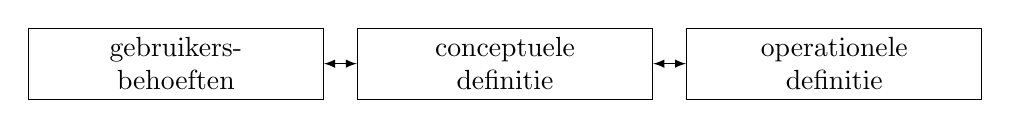
\begin{tikzpicture}[
		x=\linewidth,
		box/.style={draw,text width=10em,align=center},
		arr/.style={latex-latex}
		]
		\node[box,anchor=west] (N1) at (0,0) {gebruikers-\\behoeften};
		\node[box,anchor=center] (N2) at (0.5,0) {conceptuele\\definitie};
		\node[box,anchor=east] (N3) at (1,0) {operationele\\definitie};
		\draw[arr] (N1) to (N2);
		\draw[arr] (N2) to (N3);
	\end{tikzpicture}
\end{figure}



\paragraph{De conceptuele definitie is niet in lijn met de algemene gebruikersbehoeften}

In sommige situaties kan er een wanverhouding ontstaan tussen gebruikersbehoeften en de operationele definitie van een statistiek. Zo kunnen gebruikers bijvoorbeeld het cijfer 525\,935 systematisch interpreteren als de grootte van de verblijvende Antwerpse bevolking in plaats van de wettelijke bevolking omdat ze beleidsmatig ook voornamelijk de grootte van de verblijvende bevolking nodig hebben. In zo’n situatie spreken we van een \emph{kwaliteitsprobleem} omdat de operationele definitie van onze cijfers niet in overeenstemming is met de gebruikersbehoeften.

Voor cijfers waarbij we zo'n kwaliteitsprobleem opmerken, moeten we onderzoeken of we onze operationele definitie kunnen aanpassen aan de behoeften. In bovenstaande situatie zou het bijvoorbeeld aangeraden zijn om als Statistiek Vlaanderen voortaan Eurostat te volgen en de grootte van de verblijvende bevolking te publiceren in plaats van de wettelijke bevolking.  

\paragraph{De conceptuele definitie is niet in lijn met gebruikersbehoeften van sommige gebruikers}

In vele situaties is een evaluatie van gebruikersbehoeften en kwaliteit van een statistiek echter geen zwart-wit-verhaal. Er kunnen zich immers situaties voordoen waarin de voorgestelde operationele definitie voldoet voor de ene gebruiker maar niet voor een andere gebruiker. Zo kan onze statistiek over bevolkingsgrootte op basis van de wettelijke bevolking voldoende zijn voor heel wat gebruikers, behalve voor een speciefieke beleidsmaker die het woonbeleid in Antwerpen moet bepalen. Deze beleidsmaker heeft misschien nood aan exacte cijfers over de verblijvende bevolking in plaats van de wettelijke bevolking. Ook in zo’n geval is er een gebruikersbehoefte waar we met de statistiek ``Aantal inwoners in Antwerpen'' niet aan voldoen, ook al voldoet deze statistiek wel voor andere gebruikersbehoeften.

In situaties met verschillende niet-overlappende gebruikersbehoeften kunnen we besluiten niet langer één statistiek te publiceren maar verschillende statistieken. Zo kunnen we besluiten niet één statistiek te publiceren over ``het aantal inwoners in Antwerpen'', maar wel twee afzonderlijke statistieken: ``de wettelijke bevolkingsgrootte van Antwerpen`` en ``de verblijvende bevolkingsgrootte van Antwerpen''. We voldoen dan aan de specifieke noden van alle gebruikers. Merk op dat we in zo'n situaties zowel de conceptuele definities als de bijhorende operationele definities verder verfijnen. Uiteraard moeten dit soort keuzes steeds gebeuren vanuit praktische en pragmatische overwegingen in functie van de middelen en het personeel die we ter beschikking hebben. We kunnen in de bovenstaande situatie bijvoorbeeld ook besluiten om niet te voldoen aan de noden van deze éne speciefieke beleidsmaker omdat dit te veel energie zou vragen voor een te kleine return.

\paragraph{De operationele definitie is niet in lijn met de conceptuele definitie}

AANVULLEN


Bovenstaande situaties tonen dat het essentieel is om voor elke statistiek niet alleen de conceptuele en operationele definitie, maar ook de gebruikersbehoeften grondig in kaart te brengen. Wie gebruikt de statistieken? Welk decreet dwingt ons ertoe deze statistieken te verzamelen? Voor welke beleidsbeslissingen of welk onderzoek zijn deze statistieken relevant? \ldots? Hoewel onderzoek naar deze vragen geen exacte wetenschap is, is het noodzakelijk om de kwaliteit van statistieken te kunnen beoordelen.

We moeten ook opmerken dat kwaliteit in de brede zin van het woord kan worden bekeken. Een operationele definitie kan inhoudelijk aansluiten bij een gebruikersbehoefte, maar als de berekening te lang duurt en de statistiek te laat beschikbaar is, verlaagt dit alsnog de kwaliteit. Het is dus belangrijk een evenwicht te vinden tussen verschillende elementen van kwaliteit zoals inhoudelijke nauwkeurigheid, gebruiksvriendelijkheid en tijdige levering. Een overzicht van alle kwaliteitseisen voor statistieken wordt gegeven in de \emph{Praktijkcode voor Europese Statistieken}\footnote{zie \href{https://ec.europa.eu/eurostat/documents/4031688/9394211/KS-02-18-142-NL-N.pdf}{ec.europa.eu/eurostat/documents/4031688/9394211/KS-02-18-142-NL-N.pdf}}.

%[TOEVOEGEN: Bespreking punten praktijkcode voor Europese Statistieken: aantonen hoe elk punt neerkomt op risico voor gebruikersbehoeften en wanverhouding met operationele definitie.]
%%% Toevoegen: koppeling tussen europese praktijkcode en bovenstaande concepten. Bijvoorbeeld relevantie betekent dat er een duidelijke gebruikersbehoefte is. Deugdelijke methoden (en heel wat andere eisen uit praktijkcode) gaan eigenlijk enkel over de match tussen gebruikersbehoeften en de operationele definitie. Dit is waarom de praktijkcode niet compleet is, veel punten gaan eigenlijk over hetzelfde.

\begin{info}
	
	
	%De Europese praktijkcode bevat heel wat artikelen die echter niet relevant zijn voor het transitietraject omdat ze al worden beantwoord door de huidige afspraken binnen het SV-netwerk of door de huidige werking. Zo zijn beginsel 1 over de professionele onafhankelijkheid van de officiële statistiekproductie en beginsel 2 over het mandaat om gegevens te verzamelen reeds decretaal verankerd. Voor beginsel 11 over relevantie worden binnen de VSA reeds initiatieven genomen rond gebruikersonderzoek via verschillende thematische werkgroepen samengesteld door het Coördinatiecomité Vlaamse Openbare Statistieken (CVOS) en de Raad voor Vlaamse openbare statistieken (RVOS), die los staan van de wijze waarop we gegevens verzamelen en verwerken. Deze beginselen vormen dan ook geen rechtstreeks onderwerp van het transitietraject. 
	%De volgende beginselen vormen echter nog wel werkpunten die moeten worden aangepakt in het transitietraject:
	%•	Beginsel 4 over een sterk kwaliteitsbewustzijn
	%•	Beginsel 5 over statistische geheimhouding en gegevensbescherming
	%•	Beginsel 6 over onpartijdigheid en objectiviteit
	%•	Beginsel 7 over deugdelijke methoden
	%•	Beginsel 8 over geschikte statistische procedures
	%•	Beginsel 10 over kosteneffectiviteit
	%•	Beginsel 12 over nauwkeurigheid en betrouwbaarheid
	%•	Beginsel 14 over samenhang, vergelijkbaarheid en consistentie
	%•	Beginsel 15 over toegankelijkheid en duidelijkheid
	%De Europese praktijkcode vertalen we binnen de VSA in volgende 10 algemene doelstellingen:
	%1.	We documenteren onze data- en analyseprocessen op een transparante en afdoende manier, ter ondersteuning, optimalisering, reproduceerbaarheid en controle van onze interne processen en ter duiding van de kwaliteit van onze producten tegenover externen. 
	%2.	We verzamelen en beheren onze data met een duidelijk doel: de data die we binnen de VSA verzamelen en beheren zijn relevant voor de ontwikkeling, productie en ontsluiting van betrouwbare en kwaliteitsvolle Vlaamse openbare statistieken, door VSA of door de SV-entiteiten met ondersteuning van VSA. 
	%3.	We structureren en inventariseren onze data: we maken zichtbaar welke data beschikbaar zijn binnen de VSA en waarvoor we die data nodig hebben.
	%4.	We benutten de analysemogelijkheden van onze data optimaal en (her)gebruiken onze data intern zo veel mogelijk, met inachtneming van de regels rond het statistisch geheim.  
	%5.	We zetten in op permanente kwaliteitsverbetering van onze activiteiten via uniformisering, standaardisering, (semi-)automatisering, waarbij we gebruik maken van bestaande internationale standaarden die we op een haalbare manier vertalen naar onze organisatie.
	%6.	We maken binnen de VSA duidelijke afspraken over rollen en verantwoordelijkheden en over een efficiënte organisatie van het datamanagement, -gebruik en -analyse. We voorzien de nodige begeleiding en vorming voor de medewerkers zodat zij die afspraken kunnen implementeren. 
	%7.	We beveiligen onze data op een correcte manier, slaan ze op en bewerken ze op een binnen de VSA gedeelde omgeving (en enkel daar) en beveiligen ze zowel tegenover externen, als tegenover oneigenlijk gebruik door interne medewerkers, in lijn met de geldende AVG- en NIS2-regelgeving. 
	%8.	We beperken het aantal data- en analysetools in functie van economische en technische efficiëntie en interne expertise-ontwikkeling en bewaken de interoperabiliteit tussen de verschillende tools.
	%9.	We ontsluiten onze data tijdig, kwalitatief en afgestemd op onze verschillende gebruikersgroepen, met inachtneming van de regelgeving rond het statistisch geheim. We gaan uit van het principe ‘zo open als mogelijk, zo afgeschermd als noodzakelijk’. 
	%10.	We optimaliseren onze organisatie en werking stap voor stap en op een voor ons team haalbare manier en laten ons daarbij inspireren door de activiteiten, goede praktijken en ervaringen van andere statistiekinstellingen in binnen- en buitenland. 
\end{info}













\begin{info}
	Gebruikersbehoeften, conceptuele en operationele definitie komen weliswaar aan bod in informatiestandaarden zoals de SIMS en de GSBPM maar op een zeer onduidelijke en onoverzichtelijke manier. In de SIMS worden de gebruikersbehoeften pas opgelijst in categorie 12 terwijl dit de start vormt van een statistiekproductieproces. De operationele definitie zit in de SIMS dan weer op een zeer onsamenhangende manier verspreid over verschillende categorieën terwijl de conceptuele definitie volledig ontbreekt. 
	
	De GSBPM doet het op dit vlak beter. Het beschrijft een proces dat vertrekt vanuit gebruikersbehoeften en eindigt met een evaluatie. Het expliciteert echter onvoldoende dat de evaluatie gestoeld moet zijn op de gebruikersbehoeften en alle operationele keuzes die onderweg werden gemaakt.  
\end{info}

% Opmerking Jo: Maar we gaan nu toch verder met de SIMS als standaard voor de metadata. Of stel je dat hier in vraag?
% De SIMS kan blijven gebruikt worden. Maar ik blijf bij mijn opmerking dat we die vooral als afchecklijst moeten gebruiken en niet blindelings de structuur moeten overnemen. De structuur is chaotisch en onoverzichtelijk. Bij GSBPM zie je dat er al meer werd nagedacht over de structuur van de informatie en wordt er expliciet toegegeven dat dat maar een ideaaltype is waarvan kan worden afgeweken. De SIMS lijkt voor mij de uitkomst van een wilde brainstorm waarbij de belangrijke stap vergeten werd om alles nadien duidelijker te structureren.




























\subsection{Attributen van cijfers}


Naast de operationale definitie van een cijfer, kan een cijfer gekenmerkt worden door andere informatie, die geen betekenis geeft aan het cijfer. Dit worden \emph{attributen} genoemd.

Een belangrijke informatiepunt is de vertrouwelijkheid van het cijfer. Kan het cijfer worden gedeeld met het breed publiek, met collega's of is het vertrouwelijk en moet het veilig bewaard worden.

Een ander attribuut is de eigenaar van het cijfer. De eigenaar van een cijfer verwijst naar wie verantwoordelijk is voor dat cijfer. Deze kan 








\subsection{Samengevat}

Samengevat, voor elke statistiek die we produceren en publiceren hebben we nood aan:
\begin{enumerate}[nosep]
	\item de gebruikersbehoeften,
	\item een conceptuele definitie op basis van de gebruikersbehoeften,
	\item een operationele definitie,
	\item het cijfer, en
	\item een kwaliteitsevaluatie van de operationele definitie in functie van de gebruikersbehoeften.
\end{enumerate}
Tabel \ref{tab:voorbeeldstatistiek} vat deze basisinformatie samen aan de hand van het Antwerps voorbeeld. Als de gebruikersbehoeften van een statistiek nog niet in kaart zijn gebracht en er daardoor ook geen kwaliteitsevaluatie kan worden uitgevoerd, is de statistiek een experimentele statistiek. 

\begin{table}
	\caption{Een statistiek bestaat uit een cijfer, een conceptuele definitie die voortvloeit uit gebruikersbehoeften, en een operationele definitie die vertelt hoe het cijfer exact wordt gemeten. Een wanverhouding tussen gebruikersbehoeften en de operationele definitie bepaalt de kwaliteit van de statistiek.}
	\label{tab:voorbeeldstatistiek}
	\footnotesize
\begin{tblr}{ 
	width=\linewidth, 
	colspec={Q[l,t]X[l,t]},
	rows = {abovesep=5pt,belowsep=5pt}, 
	row{1-3,Z} = {fg=textcol,bg=maincol3}, 
	column{1} = {fg=white,bg=maincol2},
	hline{2-Y} = {white},
	hline{1,Z} = {maincol1}, 
	vline{1,Z} = {maincol1} 
	} 
Gebruikersbehoeften: & 
\begin{minipage}[t]{\linewidth}
\begin{gebruikersvoorwaarden}
\item Decreet XX.XX verwijst naar het aantal inwoners in Vlaamse gemeenten in de context van \ldots
\item Agentschap Binnenlands Bestuur publiceert cijfers over het aantal inwoners in gemeenten als \ldots
\item Academische onderzoekers vragen cijfers over het aantal inwoners in gemeenten om onderzoek te voeren over \ldots
\item \ldots 
\end{gebruikersvoorwaarden}
\end{minipage}
\\
Conceptuele definitie: & Aantal inwoners van de gemeente Antwerpen in 2019 \\
Operationele definitie: & De grootte van de wettelijke bevolking op 1 januari 2019 in de gemeente Antwerpen (Statbel NIS-code 11002 in 2019). De data worden aangeleverd door Statbel op basis van het Rijkregister van de natuurlijke personen. De wettelijke bevolking verwijst naar \ldots \\
Cijfer: & 525\,935 \\
Kwaliteitsevaluatie: & De gebruikers hebben eerder nood aan de grootte van de verblijvende bevolking in plaats van de wettelijke bevolking \\ 
\end{tblr} 
\end{table}







































\section{Statistiek als een cijferreeks}



\subsection{Wat is een statistiekreeks?}

In de vorige paragraaf werd uitgelegd hoe een statistiek verwijst naar één enkel cijfer met een bijbehorende conceptuele en operationele definitie ontstaan vanuit specifieke gebruikersbehoeften. In de praktijk produceren we echter veel statistieken met sterk overlappende gebruikersbehoeften en definities. Zo publiceren we niet alleen het aantal inwoners voor de gemeente Antwerpen, maar ook voor alle andere Vlaamse gemeenten, de drie gewesten en heel België. Aparte definities opstellen en beheren voor al deze cijfers is niet efficiënt.
% Danny: Deze definitie-cascade is onder andere een reden waarvoor GSIM deze nuances in verschillende noties probeert te vatten (en het dus helaas ook zo abstract wordt). 

Om efficiëntie te verhogen werken we daarom met \emph{statistiekreeksen} of cijferreeksen: verzamelingen van statistieken die grotendeels dezelfde conceptuele en operationele definities delen. Tabel \ref{tab:voorbeeldcijferreeks} toont bijvoorbeeld een statistiekreeks met de inwonersaantallen van alle Vlaamse gemeenten. 

\begin{table}
	\caption{We publiceren doorgaans geen individuele statistieken maar statistiekreeksen.}
	\label{tab:voorbeeldcijferreeks}
	\input{02_Wat_is_een_statistiek/tables/voorbeeldcijferreeks}
\end{table}



\subsection{Concepten, dimensies en attributen}

Aangezien de conceptuele en operationele definities van individuele cijfers in statistiekreeksen overlappen, kunnen we deze definities opsplitsen in verschillende onderdelen. Deze verschillende onderdelen van de definities worden de \emph{concepten} genoemd. Concepten zijn eigenlijk gewoon variabelen, kenmerken waar de statistieken naar refereren en die kunnen variëren tussen statistieken. Bij de statistiekreeks in tabel \ref{tab:voorbeeldcijferreeks} kunnen we bijvoorbeeld drie concepten onderscheiden: (1) de parameter ``aantal inwoners'', (2) het jaartal ``2019'', en (3) de gemeente. Niet alle statistieken die we publiceren geven immers het aantal inwoners als parameter weer, en evenmin geven ze allemaal informatie voor het jaar 2019. De statistiekreeks in tabel \ref{tab:voorbeeldcijferreeks} toont bovendien al aan hoe gemeente varieert over verschillende statistieken.

Binnen één statistiekreeks wordt een onderscheid gemaakt tussen twee soorten concepten. Sommige concepten helpen elk cijfer uniek te identificeren, terwijl anderen enkel bijkomende informatie geven over de cijfers. De concepten die de cijfers helpen identificeren binnen een statistiekreeks bepalen de \emph{dimensies} van de statistiekreeks. Ze worden ook wel \emph{identificeerders} (identifiers) genoemd. In tabel \ref{tab:voorbeeldcijferreeks} is er slechts één dimensie, namelijk de gemeente, aangezien elk cijfer het aantal inwoners van een andere gemeente weergeeft en de cijfers enkel van elkaar verschillen door de de gemeente waarnaar ze verwijzen.

De concepten die enkel bijkomende informatie geven zonder de cijfers verder te identificeren worden daarentegen \emph{attributen} genoemd. Attributen worden daarom ook soms \emph{beschrijvers} (describers) genoemd. In tabel \ref{tab:voorbeeldcijferreeks} zijn de parameter en het jaartal de attributen, omdat elk cijfer verwijst naar een inwonersaantal in 2019 en niets anders. Attributen kunnen informatie bevatten voor de hele statistiekreeks, maar kunnen evengoed enkel informatie bevatten voor één enkel cijfer of een beperkte groep van cijfers binnen de statistiekreeks. Een voorbeeld van zo’n laatste situatie is informatie over de vertrouwelijkheid van cijfers. Één groep cijfers in een tabel kan beschouwd worden als vrij te publiceren terwijl een andere groep niet openbaar mag gemaakt worden omdat ze vertrouwelijke informatie kunnen ontsluiten. De aanduiding van deze vertrouwelijkheid identificeert de cijfers op zich niet maar varieert wel van cijfer tot cijfer. 

Onthoud echter dat attributen dimensies kunnen worden wanneer verschillende statistiekreeksen worden samengevoegd. Om bijvoorbeeld bevolkingsdichtheden te berekenen, moeten de cijfers uit tabel \ref{tab:voorbeeldcijferreeks} worden gecombineerd met cijfers over de oppervlakte van alle gemeenten. In die samengestelde tabel wordt de parameter een dimensie in plaats van een attribuut, omdat sommige cijfers verwijzen naar de parameter ‘aantal inwoners’, terwijl anderen verwijzen naar de parameter ``oppervlakte'' van de gemeenten. Hetzelfde gebeurt met het concept jaartal wanneer we aantallen inwoners combineren over verschillende jaren heen voor een tijdreeks. Omgekeerd kan een dimensie ook een attribuut worden wanneer we een tabel opsplitsen volgens die dimensie. Bijvoorbeeld, als we longitudinale data op jaarbasis opsplitsen in aparte tabellen per jaartal, wordt jaartal in die nieuwe tabellen slechts een attribuut in plaats van een dimensie. Het verschil tussen attributen en dimensies is dus relatief want het hangt af van welke tabel je precies bekijkt. Over al mogelijke statistieken bekeken zijn alle concepten dimensies want geen enkele operationele definitie is dezelfde.

\begin{info}
	We hebben hier een hiaat in het SDMX model blootgelegd. De documentatie van SDMX bespreekt nergens hoe attributen dimensies kunnen worden of vice versa wanneer datasets met statistiekreeksen worden samengevoegd of uitgesplitst. Om deze reden is de uitwerking van attributen in het model ook veel beperkter dan de uitwerking van dimensies. Hierdoor kan SDMX moeilijker gelinkt worden aan de ideeën rond conceptuele definities, operationele definities en kwaliteit van statistiekreeksen.
	
	Sterker nog, binnen SDMX wordt parameter nooit duidelijk beschouwd als een dimensie waardoor je verschillende parameters zoals bevolkingsgrootte en oppervlakte moeilijk in één tabel kan combineren zonder in problemen te komen over de definitie van dimensies en attributen.
\end{info}





\subsection{Conceptuele en operationele definitie}

Net zoals elke afzonderlijke statistiek worden statistiekreeksen ook beschreven via een conceptuele en een operationele definitie. Dit vergemakkelijkt informatiebeheer over de statistiekreeksen.

De \emph{conceptuele definitie} verwijst naar de interpretatie die een doorsnee gebruiker aan de statistiekreeks toekent. De statistiekreeks in tabel \ref{tab:voorbeeldcijferreeks} kan bijvoorbeeld conceptueel worden gedefinieerd als het ``aantal inwoners in gemeenten in het Vlaamse Gewest in 2019''. Deze definitie sluit aan bij specifieke gebruikersbehoeften, zoals bijvoorbeeld beschreven in tabel \ref{tab:voorbeeldstatistiek}.

De \emph{operationele definitie} van een statistiekreeks beschrijft hoe de cijferreeks pre‐ cies werd verzameld en gereproduceerd kan worden. Bovendien specificeert de operationele definitie steeds welke waarden de attributen en dimensies binnen de reeks precies aannemen. Voor tabel \ref{tab:voorbeeldcijferreeks} luidt de operationele definitie bijvoorbeeld: ``De grootte van de wettelijke bevolking op 1 januari 2019 per gemeente volgens de NIS‐code‐indeling in 2019. De wettelijke bevolking omvat\ldots '' Deze definitie benoemt heel duidelijk ‘gemeente’ als dimensie en geeft aan hoeveel gemeenten de reeks omvat, namelijk de 300 Vlaamse gemeenten volgens de NIS‐code‐indeling van 2019, en bijvoorbeeld niet de 285 Vlaamse gemeenten vanaf 2025. Daarnaast beschrijft de definitie ook heel duidelijk de waarde van de attributen. De reeks bevat namelijk cijfers over de grootte van de wettelijke bevolking en bijvoorbeeld niet de verblijvende bevolking, en voor het jaar 2019 en geen ander kalenderjaar.

Door de exacte beschrijving van dimensies bepaalt de operationele definitie bovendien strikt uit hoeveel cijfers een statistiekreeks bestaat, zelfs als sommige cijfers een missende of versluierde waarde hebben. De reeks in tabel \ref{tab:voorbeeldcijferreeks} bestaat bijvoorbeeld uit 300 cijfers, voor elke Vlaamse gemeente één. Als er in de reeks ook totaalcijfers zouden worden gepubliceerd voor Vlaanderen, Wallonië, Brussel en België, verandert de dimensie ‘gemeente’ naar het ruimer concept ‘geografisch gebied’ met 304 mogelijke waarden en dikt de reeks tot evenveel cijfers aan. Splitsen we de cijfers verder uit naar mannen en vrouwen, dan wordt de dimensie ‘geslacht’ toegevoegd met twee mogelijke waarden (man en vrouw) en bevat de reeks plots 608 cijfers. Inclusief de totalen over beide geslachten komt het totaal op 912 cijfers. Voeg daar nog het percentage mannen en vrouwen per gemeente aan toe, dan bevat de reeks 1520 cijfers.

Een kleine tip om de operationele definitie duidelijk uit te schrijven: Maak slim gebruik van voorzetsels zoals ``voor'', ``in'' of ``per'' om de attributen en dimensies aan te duiden. Zo kan je bijvoorbeeld een statistiekreeks definiëren als het ``aantal inwoners IN het jaar 2019 PER geografisch gebied (Vlaamse gemeenten, Belgische gewesten en heel België volgens de NIS‐code‐indeling van 2019), VOOR elk geslacht (mannen, vrouwen, totaal), en PER leeftijdsgroep (0‐18, 19‐30, 31‐65, 66+ jaar, totaal).'' 
% Hier dieper op ingaan in een aparte paragraaf?

Hoewel het bij de conceptuele definitie minder strikt is om alle attributen en dimensies expliciet te vermelden, is dit ook een goede praktijk. Voor de statistiekreeks in tabel \ref{tab:voorbeeldcijferreeks} kunnen we bijvoorbeeld kiezen tussen de conceptuele definities ``bevolkingsomvang'' of ``aantal inwoners in de Vlaamse gemeenten in 2019''. De tweede definitie is uiteraard een pak duidelijker als omschrijving. De eerste definitie is anderzijds een pak beknopter en gemakkelijker te citeren maar wordt uiteraard dubbelzinnig als we ook tabellen publiceren voor andere kalenderjaren (tenzij we al deze tabellen samenvoegen natuurlijk, maar dan zitten we weer in een ander verhaal).

%%% AANPASSEN: Conceptuele definitie moet wel verwijzing hebben naar dimensies. In de gebruikersbehoeften moet immers ook naar voor komen waarom cijfers over de dimensies nodig zijn, anders zijn de statistieken niet relevant => lage kwaliteit. De dimensies moeten ook geoperationaliseerd worden van conceptuele naar operationele definitie. Bijvoorbeeld, in de conceptuele definitie staat `cijfers per gemeente', in de operationele definitie moet dan staan welke opdeling van gemeenten precies bedoeld worden.


Net zoals bij individuele statistieken bepaalt een wanverhouding tussen gebruikersbehoeften en de operationele definitie mee de kwaliteit van een statistiekreeks. Als de operationele definitie niet in lijn ligt met de behoeften van gebruikers moet de reeks worden aangepast of worden geschrapt.

De presentatie van een statistiekreeks gebeurt doorgaans niet zoals in tabel \ref{tab:voorbeeldcijferreeks}. Attributen worden vaak uit de rijen verwijderd en opgenomen in de titel of conceptuele definitie van de statistiekreeks. Tabel \ref{tab:voorbeeldcijferreeks2} toont een meer gangbare weergave van een uitgebreidere cijferreeks. In deze tabel zie je dat de concepten ``aantal inwoners'' en jaartal ``2019'' enkel worden vermeld in de titel van de tabel. De tabel telt verder drie dimensies. Dimensies gemeente en geslacht staan in de rijen. De derde dimensie is de statistische parameter die een verschil maakt tussen aantallen en percentages. Deze dimensie staat in de kolommen.

\begin{table}
	\caption{De conceptuele definitie van een statistiekreeks verwijst naar de interpretatie van een doorsnee gebruiker terwijl de operationele definitie alle concepten (attributen en dimensies) van de reeks duidelijk beschrijft.}
	\label{tab:voorbeeldcijferreeks2}
	\footnotesize
\begin{tblr}{
	width=\linewidth,
	colspec={X[c]X[c]X[c]X[c]},
	column{1-2} = {fg=textcol,bg=maincol3},
	row{1} = {fg=white,bg=maincol1},
	row{2} = {fg=white,bg=maincol2},
	hline{1,Z} = {maincol1},
	vline{1,Z} = {maincol1},
	hspan=minimal
	}
\SetCell[c=4]{l} \parbox{\linewidth}{\MakeUppercase{Aantal mannen en vrouwen in Vlaamse gemeenten in 2019.} \\ Het aantal en het percentage mannen en vrouwen in de wettelijke bevolking op 1 januari 2019 per gemeente volgens de NIS-code-indeling in 2019.} \\
Gemeente & Geslacht & Aantal & Percentage \\
Aartselaar & man & 7089 & 49.6 \\
Aartselaar & vrouw & 7204 & 50.4 \\
Antwerpen & man & 262921 & 50.0 \\
Antwerpen & vrouw & 263014 & 50.0 \\
Boechout & man & 6506 & 49.0 \\
Boechout & vrouw & 6760 & 51.0 \\
Boom & man & 9024 & 49.5 \\
Boom & vrouw & 9220 & 50.5 \\
Borsbeek & man & 5270 & 48.6 \\
Borsbeek & vrouw & 5584 & 51.4 \\
\end{tblr}
\end{table}

\begin{info}
	Binnen de huidige SDMX-standaard stellen we statistiekreeksen voor met slechts één kolom voor de cijfers. De structuur in tabel \ref{tab:voorbeeldcijferreeks} zou hiervoor gepivoteerd moeten worden. Hoogstwaarschijnlijk versoepelt de SDMX-standaard echter in de toekomst waardoor verschillende kolommen cijfers kunnen bevatten. 
\end{info}





















\subsection{Samengevat}

Samengevat, een statistiekreeks is een reeks van statistieken waarbij gebruikersbehoeften, conceptuele en operationele definities overlappen. Elke statistiekreeks is nauwkeurig gedefinieerd via haar operationele definitie. Deze operationele definitie vertelt exact hoeveel cijfers de statistiekreeks bevat, wat deze cijfers betekenen en hoe de cijfers werden bekomen. Een wanverhouding tussen de operationele definitie en de gebruikersbehoeften is een van de kwaliteitsindicatoren van de statistiekreeks volgens de praktijkcode.

Met Statistiek Vlaanderen leggen we op voorhand vast welke statistiekreeksen we publiceren. Deze statistiekreeksen zijn terug te vinden in het Vlaams Statistisch Programma (VSP‐lijst). Voor elke statistiek in de VSP‐lijst voorzien we ten minste volgende informatie:   
% JO: Wat er in de VSP-lijst moet staan ligt vast door afspraken met IIS. Info die je voorstelt zou ik opnemen in SIMS-medata.
\begin{enumerate}[nosep]
	\item de conceptuele definitie (die gebruikt wordt als handig label voor de statistiekreeks),
	\item het versienummer
	\item de operationele definitie inclusief een beschrijving van alle concepten (attributen en dimensies) inclusief de exacte waarden van die concepten,
	\item een overzicht van de gebruikersbehoeften, en
	\item een kwaliteitsevaluatie van de operationele definitie in functie van de gebruikersbehoeften.
\end{enumerate}
Tabel \ref{tab:voorbeeldVSPlijst} toont hoe de VSP-lijst er minimaal zou moeten uitzien. In de praktijk zullen we uiteraard informatie over statistiekreeksen niet bewaren in één gigantische tabel maar werken met informatiefiches per statistiekreeks gebaseerd op de   single integrated metadata structure (SIMS)\footnote{\href{https://ec.europa.eu/eurostat/web/metadata/reference-metadata-reporting-standards}{ec.europa.eu/eurostat/web/metadata/reference-metadata-reporting-standards}}.

\begin{table}
	\caption{Het Vlaams Statistisch Programma (VSP) definieert een lijst van statistiekreeksen die Statistiek Vlaanderen publiceert. Elke statistiekreeks in deze reeks beschikt over een duidelijke conceptuele en operationele definitie, opgelijste gebruikersbehoeften en een kwaliteitsevaluatie.}
	\label{tab:voorbeeldVSPlijst}
	\begin{mdframed}
\newlist{reeks}{description}{1}
\setlist[reeks]{
	font=\bfseries\color{maincol1},
	labelindent=0pt,
	labelwidth=3ex,
	labelsep=1ex,
	itemindent=0pt,
	leftmargin=!,
	itemsep=2\baselineskip
	}
\newlist{features}{description}{1}
\setlist[features]{
	nosep,
	font=\mdseries\itshape\color{maincol2},
	labelindent=0pt,
	labelwidth=3ex,
	labelsep=1ex,
	itemindent=0pt,
	leftmargin=!
	}
\tiny
\begin{reeks}
\item[Aantal mannen en vrouwen, versie 1] \mbox{}
	\begin{features}
	\item[gebruikersvoorwaarden:] \mbox{}
		\begin{gebruikersvoorwaarden}
		\item Decreet XX.XX verwijst naar het aantal inwoners in Vlaamse gemeenten om beleid te voeren over \ldots
		\item Agentschap Binnenlands Bestuur publiceert cijfers over het aantal inwoners in gemeenten als \ldots
		\item Academische onderzoekers vragen cijfers over het aantal inwoners in gemeenten om onderzoek te voeren over \ldots
		\item \ldots 
		\end{gebruikersvoorwaarden}
	\item[Operationele definitie:]
	Het aantal en het percentage mannen en vrouwen in de feitelijke bevolking (aantal geregistreerde inwoners in het Rijksregister inclusief personen in het wachtregister en ambassadeurs) op 1 januari van elk kalenderjaar vanaf 2005 per Vlaamse gemeente volgens de NIS-code-indeling in 2019 = 600 cijfers per jaar.
	\item[Kwaliteit:]
	De gebruikers hebben eerder nood aan de grootte van de verblijvende bevolking in plaats van de feitelijke bevolking.
	\item[Nota:] Stopgezet in 2022, wegens aanpassing definitie.
	\end{features}
\item[Aantal mannen en vrouwen, versie 2] \mbox{}
	\begin{features}
	\item[gebruikersvoorwaarden:] \mbox{}
		\begin{gebruikersvoorwaarden}
		\item Decreet XX.XX verwijst naar het aantal inwoners in Vlaamse gemeenten om beleid te voeren over \ldots
		\item Agentschap Binnenlands Bestuur publiceert cijfers over het aantal inwoners in gemeenten als \ldots
		\item Academische onderzoekers vragen cijfers over het aantal inwoners in gemeenten om onderzoek te voeren over \ldots
		\item \ldots 
		\end{gebruikersvoorwaarden}
	\item[Operationele definitie:]
	Het aantal en het percentage mannen en vrouwen in de verblijvende bevolking (aantal geregistreerde inwoners in het Rijksregister inclusief personen in het wachtregister en ambassadeurs en personen die minder dan drie maanden in België verblijven) op 1 januari van elk kalenderjaar vanaf 2005 per Vlaamse gemeente volgens de NIS-code-indeling in 2019 = 600 cijfers per jaar. 
	\item[Kwaliteit:] Onderzoek XX toont aan dat er geen problemen zijn met deze statistiekreeks. 
	\item[Nota:] Stopgezet in 2025, wegens aanpassing gemeenten door fusies.
	\end{features}
\item[Aantal mannen en vrouwen, versie 3] \mbox{}
	\begin{features}
	\item[gebruikersvoorwaarden:] \mbox{}
		\begin{gebruikersvoorwaarden}
		\item Decreet XX.XX verwijst naar het aantal inwoners in Vlaamse gemeenten om beleid te voeren over \ldots
		\item Agentschap Binnenlands Bestuur publiceert cijfers over het aantal inwoners in gemeenten als \ldots
		\item Academische onderzoekers vragen cijfers over het aantal inwoners in gemeenten om onderzoek te voeren over \ldots
		\item \ldots 
		\end{gebruikersvoorwaarden}
	\item[Operationele definitie:]
	Het aantal en het percentage mannen en vrouwen in de verblijvende bevolking (aantal geregistreerde inwoners in het Rijksregister inclusief personen in het wachtregister en ambassadeurs en personen die minder dan drie maanden in België verblijven) op 1 januari van elk kalenderjaar vanaf 2005 per Vlaamse gemeente volgens de NIS-code-indeling in 2025 = 570 cijfers per jaar. 
	\item[Kwaliteit:]
	Onderzoek XX toont aan dat er geen problemen zijn met deze statistiekreeks.  
	\end{features}
\item[Tewerkstelling in hoogtechnologische sector, versie 1] \mbox{}
	\begin{features}
	\item[gebruikersvoorwaarden:] \mbox{}
		\begin{gebruikersvoorwaarden}
		\item Decreet XX.XX verwijst naar Tewerkstelling in hoogtechnologische sector in kader van \ldots
		\item De cijferpagina met cijfers over tewerkstelling in hoogtechnologische sector wordt X aantal keer per jaar geraadpleegd.
		\item \ldots
		\end{gebruikersvoorwaarden}	
	\item[Operationele definitie:] Percentage van de hele werkende bevolking aan de slag in de hoogtechnologische sector op 1 januari van elk kalenderjaar vanaf 2005 per Vlaamse gemeente en voor het hele VLaamse gewest volgens de NIS-code-indeling in 2019. De werkende bevolking omhelst \ldots De hoogtechnologische sector bestaat uit- bedrijven \ldots De data worden verzameld via de Enquête naar de Arbeidskrachten (EAK) door Statbel. In deze enquête wordt data verzameld door \ldots = 301 cijfers per jaar.
	\item[Kwaliteit:]
	Onderzoek YY toont aan dat er geen problemen zijn met deze statistiekreeks. 
	\end{features}
\item[Drinkwaterkwaliteit, versie 1] \mbox{}
	\begin{features}
	\item[gebruikersvoorwaarden:] \mbox{}
		\begin{gebruikersvoorwaarden}
		\item Decreet XX.XX verwijst naar drinkwaterkwaliteit in kader van \ldots
		\item \ldots
		\end{gebruikersvoorwaarden}
	\item[Operationele definitie:] Conformiteitspercentage van het kraantjeswater in heel Vlaanderen per jaar. Het conformiteitspercentage wordt berekend door Vlaamse Milieumaatschappij (VMM) op basis van het totale aantal analyses en het totale aantal vastgestelde normoverschrijdingen voor volgende parameters: \ldots = 1 cijfer per jaar.
	\item[Kwaliteit:]
	Volgens rapport ZZ ontstaan er kleine onzekerheidsfouten in de meting van parameter x, waardoor het werkelijke conformiteitspercentage kan afwijken met 0,2\%. Deze fluctuatie heeft slechts beperkte invloed op de kwaliteit waardoor geen herdefiniëring nodig is.
	\end{features}
\item[\ldots\ldots\ldots, versie \ldots] \mbox{}
	\begin{features}
	\item[gebruikersvoorwaarden:] \ldots
	\item[Operationele definitie:] \ldots
	\item[Kwaliteit:]\ldots	
	\end{features}
\item[\ldots\ldots\ldots]
\end{reeks}
\end{mdframed}
\end{table}
























\section{Statistiek als een tabelreeks}


Voorbeeld: bevolking naar leeftijd en geslacht --- bevolkingspyramide
Hieruit kunnen heel wat andere cijferreeksen worden berekend
- aantal inwoners naar geslacht
- percentage volgens geslacht
- aantal inwoners naar leeftijd
- percentage per leeftijd
- percentage 65+'ers
- vergrijzing
- \ldots

Opnieuw conceptuele en operationele definitie nodig




















\section{Experimentele statistieken}

% experimentele statistiek: start van eurostat, daaruit verschillende opties: zowel geen behoefte, maar ook anders wel een behoefte, maar testen van bron, methode om iets te meten en dan te kijken of het voldoet aan de gebruikersbehoeften


Sommige statistieken ontstaan niet vanuit geobserveerde gebruikersbehoeften, maar vanuit veronderstellingen hierover. Dit kan voortkomen uit de inhoudelijke interesse van een collega of door nieuwe dataverzamelings‐ of analysemethoden. Deze statistieken noemen we \emph{experimentele statistieken}. 

% JO: Experimentele statistieken zijn voor mij statistieken ontwikkeld op basis van innovatieve methoden of bronnen. Dat is voor mij niet verbonden met al dan niet bestaan van gebruikersvraag. Een gebruikersvraag kan zo complex zijn om te operationaliseren dat daarvoor nieuwe technieken nodig of bruikbaar kunnen zijn.
% Zie ook definitie van Eurostat: Experimental statistics use new data sources and methods to better respond to our users' needs in a timely manner. Zie: https://ec.europa.eu/eurostat/web/experimental-statistics
% JORRE: We kunnen de statistieken in de tekst ook een andere naam geven, maar we gaan ze op de één of andere manier toch moeten benoemen.
% De Eurostat definitie is trouwens rekbaar, als wij een nieuwe statistiek invoeren, bijvoorbeeld, op basis van een nieuwe eenvoudige vraag in de SV-bevraging, is dat ook een “nieuwe data-bron”, hoewel jij dat waarschijnlijk niet als innovatief zal bestempelen. Zo zijn alle statistieken, waarvoor we geen opgelijste gebruikersbehoeften hebben, ooit ontstaan uit een nieuwe databron. ‘Nieuwe databron’ in de zin dat we de bron daarvoor niet gebruikten om statistieken aan te maken.
% Sowieso heb je voor beide groepen statistieken, experimentele statistieken en statistieken waarvoor we geen duidelijke gebruikersbehoeften hebben, dezelfde aanpak nodig. We maken ze aan omdat we denken dat ze nuttig zijn maar zonder duidelijke gebruikersbehoeften in kaart te hebben. Nadien moeten we voor beide categorieën evalueren of ze nuttig zijn voor gebruikers. Mijn suggestie is om het ons dan niet moeilijk te maken en deze gewoon allemaal onder dezelfde term te categoriseren: “experimentele statistieken”


% DANNY: Vraag is dus of deze statistieken experimenteel zijn in de zin dat ze ‘nog niet officieel’ aanvaard zijn (in één of ander Statistisch Programma) of dat we ‘nieuwe ‘methodes gebruiken om tot de statistiek te komen. Ik vind het vanuit systeemontwerp alvast wel relevant om hier een éénduidig en gedragen begrip rond te creëren. Wanneer het namelijk zou betekenen dat deze statistiek productie nog ‘in een experimentele fase of status zit’ gelden hier vanuit een governance en publicatie oogpunt mogelijk ook minder stricte regels en moeten we voor de uitvoering hiervan omgevingen met meer vrijheid bieden.

Experimentele statistieken verwijzen dus niet enkel naar statistieken ontwikkeld met de allernieuwste analysetechnieken die recent op de markt werden gebracht. Eurostat definieert experimentele statistieken als ``Experimental statistics use new data sources and methods to better respond to our users' needs in a timely manner.'' Wat ``new data sources and methods'' betekent in deze definitie is echter rekbaar. Zo kan een nieuwe vraag in een bevraging al beschouwd worden als een nieuwe databron en kunnen we deze vraag gebruiken om een nieuwe experimentele statistiek te ontwikkelen waarover we enkel aannames kunnen maken over de gebruikersbehoeften.

Bij gebrek  aan concrete gebruikersbehoeften kan de kwaliteit van experimentele statistieken uiteraard niet meteen worden geëvalueerd. Kwaliteit  verwijst immers, zoals eerder al aangehaald, naar de overeenkomst tussen de gebruikersbehoeften en de operationele definitie van een statistiek. 

% LISA: Ik interpreteer kwaliteit toch ook nog op andere manieren; correct gemeten, meet het wat het moet meten,.. n

Daarom is het noodzakelijk om voor elke experimentele statistiek een deadline voor evaluatieonderzoek rond gebruikersbehoeften af te spreken (bijvoorbeeld vijf jaar na de eerste publicatie). Dit evaluatieonderzoek beantwoordt vragen zoals:
\begin{itemize}[nosep]
	\item Wordt de statistiek gebruikt, en zo ja, waarvoor?
	\item Sluit het gebruik en de interpretatie aan bij de operationele definitie?
	\item Zijn er suggesties van gebruikers om de statistiek beter af te stemmen op hun behoeften? 
\end{itemize}

Eens gebruikersbehoeften in kaart zijn gebracht, kan de kwaliteit van de statistiek verder worden geëvalueerd. Afhankelijk van de resultaten kan de statistiek nadien:
\begin{itemize}[nosep]
	\item worden geüpgraded tot een volwaardige officiële statistiek;
	\item worden aangepast op basis van de bevindingen; of
	\item worden stopgezet indien de kwaliteit onvoldoende is.
\end{itemize}

\begin{info}
	Het groot deel van de statistieken van de VSA zijn vermoedelijk experimenteel, aangezien gebruikersbehoeften niet systematisch zijn vastgelegd. Hierdoor is een kwaliteitsbeoordeling van deze statistieken momenteel moeilijk. Onderzoek naar gebruikersbehoeften dringt zich op bij deze statistieken.
\end{info}

% Opmerking Jo: De VOS’en zijn vastgelegd in de beginjaren van de VSA in overleg met de gebruikers in themagroepen. Zij voldoen dus wel aan gebruikersbehoeften. Ook nu wordt met de bepaling van de nieuwe VSP-lijst volop rekening gehouden met gebruikersbehoeften.
% JORRE: Als dat zo is, des te beter. Maar ik heb tot nu toe voor geen enkele statistiek al een overzicht van die gebruikersbehoeften gezien. Ik heb de demografen vorige week gevraagd naar de argumenten waarom we cijfers publiceren over de stand van de bevolking. Zij konden die niet geven... Tom en ik zullen die nochtans nodig hebben om de kwaliteit van de statistieken te beoordelen.




%Alle onderzoeks- en innovatieprojecten van de VSA worden geïntegreerd in een gecentraliseerde werking. Het gaat hierbij om zowel inhoudelijk verdiepend onderzoek, beleidsdomeinoverschrijdend onderzoek, onderzoek rond statistiekontwikkeling, onderzoek in het kader van academische samenwerking of data science-projecten. De activiteiten van deze groep zijn wel steeds gericht op de (verkenning van de) ontwikkeling van nieuwe openbare statistieken of de verbetering van bestaande statistieken. Daarnaast is er binnen deze werking ook plaats voor onderzoek naar efficiëntere manieren om de opdrachten en interne processen van de VSA uit te voeren (bv. experimenten met nieuwe analyse- of visualisatiesoftware). 
%De werking rond onderzoek en innovatie neemt volgende taken voor haar rekening:
%•	Organisatie van de redactieraad. Bij voorkeur mondt elk onderzoeks- of innovatieproject minstens uit in een rapport.
%•	Organisatie van (interne) seminaries waarbij onderzoek wordt voorgesteld aan de collega’s en andere geïnteresseerden.
%•	Organisatie van de data science-projecten
%•	Organisatie van de academische samenwerking zoals de ondersteuning van thesisstudenten.

















\end{document}